\documentclass[CJK]{beamer}
\usepackage{CJKutf8}
\usepackage{beamerthemesplit}
\usetheme{Malmoe}
\useoutertheme[footline=authortitle]{miniframes}
\usepackage{amsmath}
\usepackage{amssymb}
\usepackage{graphicx}
\usepackage{eufrak}
\usepackage{color}
\usepackage{slashed}
\usepackage{simplewick}
\usepackage{tikz}
\usepackage{tcolorbox}
\graphicspath{{../figures/}}
%%figures
\def\lfig#1#2{\includegraphics[width=#1 in]{#2}}
\def\addfig#1#2{\begin{center}\includegraphics[width=#1 in]{#2}\end{center}}
\def\wulian{\includegraphics[width=0.18in]{emoji_wulian.jpg}}
\def\bigwulian{\includegraphics[width=0.35in]{emoji_wulian.jpg}}
\def\bye{\includegraphics[width=0.18in]{emoji_bye.jpg}}
\def\bigbye{\includegraphics[width=0.35in]{emoji_bye.jpg}}
\def\huaixiao{\includegraphics[width=0.18in]{emoji_huaixiao.jpg}}
\def\bighuaixiao{\includegraphics[width=0.35in]{emoji_huaixiao.jpg}}
\def\jianxiao{\includegraphics[width=0.18in]{emoji_jianxiao.jpg}}
\def\bigjianxiao{\includegraphics[width=0.35in]{emoji_jianxiao.jpg}}
%% colors
\def\blacktext#1{{\color{black}#1}}
\def\bluetext#1{{\color{blue}#1}}
\def\redtext#1{{\color{red}#1}}
\def\darkbluetext#1{{\color[rgb]{0,0.2,0.6}#1}}
\def\skybluetext#1{{\color[rgb]{0.2,0.7,1.}#1}}
\def\cyantext#1{{\color[rgb]{0.,0.5,0.5}#1}}
\def\greentext#1{{\color[rgb]{0,0.7,0.1}#1}}
\def\darkgray{\color[rgb]{0.2,0.2,0.2}}
\def\lightgray{\color[rgb]{0.6,0.6,0.6}}
\def\gray{\color[rgb]{0.4,0.4,0.4}}
\def\blue{\color{blue}}
\def\red{\color{red}}
\def\green{\color{green}}
\def\darkgreen{\color[rgb]{0,0.4,0.1}}
\def\darkblue{\color[rgb]{0,0.2,0.6}}
\def\skyblue{\color[rgb]{0.2,0.7,1.}}
%%control
\def\be{\begin{equation}}
\def\ee{\nonumber\end{equation}}
\def\bea{\begin{eqnarray}}
\def\eea{\nonumber\end{eqnarray}}
\def\bch{\begin{CJK}{UTF8}{gbsn}}
\def\ech{\end{CJK}}
\def\bitem{\begin{itemize}}
\def\eitem{\end{itemize}}
\def\bcenter{\begin{center}}
\def\ecenter{\end{center}}
\def\bex{\begin{minipage}{0.2\textwidth}\includegraphics[width=0.6in]{jugelizi.png}\end{minipage}\begin{minipage}{0.76\textwidth}}
\def\eex{\end{minipage}}
\def\chtitle#1{\frametitle{\bch#1\ech}}
\def\bmat#1{\left(\begin{array}{#1}}
\def\emat{\end{array}\right)}
\def\bcase#1{\left\{\begin{array}{#1}}
\def\ecase{\end{array}\right.}
\def\bmini#1{\begin{minipage}{#1\textwidth}}
\def\emini{\end{minipage}}
\def\tbox#1{\begin{tcolorbox}#1\end{tcolorbox}}
\def\pfrac#1#2#3{\left(\frac{\partial #1}{\partial #2}\right)_{#3}}
%%symbols
\def\bropt{\,(\ \ \ )}
\def\sone{$\star$}
\def\stwo{$\star\star$}
\def\sthree{$\star\star\star$}
\def\sfour{$\star\star\star\star$}
\def\sfive{$\star\star\star\star\star$}
\def\rint{{\int_\leftrightarrow}}
\def\roint{{\oint_\leftrightarrow}}
\def\stdHf{{\textit{\r H}_f}}
\def\deltaH{{\Delta \textit{\r H}}}
\def\ii{{\dot{\imath}}}
\def\skipline{{\vskip0.1in}}
\def\skiplines{{\vskip0.2in}}
\def\lagr{{\mathcal{L}}}
\def\hamil{{\mathcal{H}}}
\def\vecv{{\mathbf{v}}}
\def\vecx{{\mathbf{x}}}
\def\vecy{{\mathbf{y}}}
\def\veck{{\mathbf{k}}}
\def\vecp{{\mathbf{p}}}
\def\vecn{{\mathbf{n}}}
\def\vecA{{\mathbf{A}}}
\def\vecP{{\mathbf{P}}}
\def\vecsigma{{\mathbf{\sigma}}}
\def\hatJn{{\hat{J_\vecn}}}
\def\hatJx{{\hat{J_x}}}
\def\hatJy{{\hat{J_y}}}
\def\hatJz{{\hat{J_z}}}
\def\hatj#1{\hat{J_{#1}}}
\def\hatphi{{\hat{\phi}}}
\def\hatq{{\hat{q}}}
\def\hatpi{{\hat{\pi}}}
\def\vel{\upsilon}
\def\Dint{{\mathcal{D}}}
\def\adag{{\hat{a}^\dagger}}
\def\bdag{{\hat{b}^\dagger}}
\def\cdag{{\hat{c}^\dagger}}
\def\ddag{{\hat{d}^\dagger}}
\def\hata{{\hat{a}}}
\def\hatb{{\hat{b}}}
\def\hatc{{\hat{c}}}
\def\hatd{{\hat{d}}}
\def\hatN{{\hat{N}}}
\def\hatH{{\hat{H}}}
\def\hatp{{\hat{p}}}
\def\Fup{{F^{\mu\nu}}}
\def\Fdown{{F_{\mu\nu}}}
\def\newl{\nonumber \\}
\def\vece{\mathrm{e}}
\def\calM{{\mathcal{M}}}
\def\calT{{\mathcal{T}}}
\def\calR{{\mathcal{R}}}
\def\barpsi{\bar{\psi}}
\def\baru{\bar{u}}
\def\barv{\bar{\upsilon}}
\def\qeq{\stackrel{?}{=}}
\def\torder#1{\mathcal{T}\left(#1\right)}
\def\rorder#1{\mathcal{R}\left(#1\right)}
\def\contr#1#2{\contraction{}{#1}{}{#2}#1#2}
\def\trof#1{\mathrm{Tr}\left(#1\right)}
\def\trace{\mathrm{Tr}}
\def\comm#1{\ \ \ \left(\mathrm{used}\ #1\right)}
\def\tcomm#1{\ \ \ (\text{#1})}
\def\slp{\slashed{p}}
\def\slk{\slashed{k}}
\def\calp{{\mathfrak{p}}}
\def\veccalp{\mathbf{\mathfrak{p}}}
\def\Tthree{T_{\tiny \textcircled{3}}}
\def\pthree{p_{\tiny \textcircled{3}}}
\def\dbar{{\,\mathchar'26\mkern-12mu d}}
\def\erf{\mathrm{erf}}
\def\const{\mathrm{constant}}
\def\pheat{\pfrac p{\ln T}V}
\def\vheat{\pfrac V{\ln T}p}
%%units
\def\fdeg{{^\circ \mathrm{F}}}
\def\cdeg{^\circ \mathrm{C}}
\def\atm{\,\mathrm{atm}}
\def\angstrom{\,\text{\AA}}
\def\SIL{\,\mathrm{L}}
\def\SIkm{\,\mathrm{km}}
\def\SIyr{\,\mathrm{yr}}
\def\SIGyr{\,\mathrm{Gyr}}
\def\SIV{\,\mathrm{V}}
\def\SImV{\,\mathrm{mV}}
\def\SIeV{\,\mathrm{eV}}
\def\SIkeV{\,\mathrm{keV}}
\def\SIMeV{\,\mathrm{MeV}}
\def\SIGeV{\,\mathrm{GeV}}
\def\SIcal{\,\mathrm{cal}}
\def\SIkcal{\,\mathrm{kcal}}
\def\SImol{\,\mathrm{mol}}
\def\SIN{\,\mathrm{N}}
\def\SIHz{\,\mathrm{Hz}}
\def\SIm{\,\mathrm{m}}
\def\SIcm{\,\mathrm{cm}}
\def\SIfm{\,\mathrm{fm}}
\def\SImm{\,\mathrm{mm}}
\def\SInm{\,\mathrm{nm}}
\def\SImum{\,\mathrm{\mu m}}
\def\SIJ{\,\mathrm{J}}
\def\SIW{\,\mathrm{W}}
\def\SIkJ{\,\mathrm{kJ}}
\def\SIs{\,\mathrm{s}}
\def\SIkg{\,\mathrm{kg}}
\def\SIg{\,\mathrm{g}}
\def\SIK{\,\mathrm{K}}
\def\SImmHg{\,\mathrm{mmHg}}
\def\SIPa{\,\mathrm{Pa}}



\newcommand{\field}{\mathscr{F}}

\newcommand{\reals}{\mathbb{R}}
\newcommand{\complexs}{\mathbb{C}}
\newcommand{\ints}{\mathbb{Z}}
%\newcommand{\dim}{\mathrm{dim\ }}
\newcommand{\diag}{\mathrm{diag \ }}
\newcommand{\up}{\uparrow}
\newcommand{\down}{\downarrow}
\newcommand{\su}{\mathfrak{su}}
\newcommand{\so}{\mathfrak{so}}
\newcommand{\tr}{\mathrm{tr\ }}

\newtheorem{thm}{定理}[section]
\newtheorem{axm}{公理}[section]
\newtheorem{dfn}{定义}[section]

%\cpic{<尺寸>}{<文件名>}}用于生成居中的图片。
\newcommand{\cpic}[2]{
\begin{center}
\includegraphics[scale=#1]{#2}
\end{center}
}

%\cpicn{<尺寸>}{<文件名>}{<注释>}用于生成居中且带有注释的图片,其label为图片名。
\newcommand{\cpicn}[3]
{
\begin{figure}[h!]
\cpic{#1}{#2}
\caption{#3\label{#2}}
\end{figure}
}

\title{Group Theory\\ Talk 1-Introduction and Discrete Groups}
  \author{}
  \date{}


\begin{document}

\begin{frame}
 
\begin{center}
\begin{Large}
\bch
Group Theory

{\vskip 0.3in}

Talk 1-Introduction and Discrete Groups

\ech
\end{Large}
\end{center}

\vskip 0.2in


\end{frame}

\section{Book}
\begin{frame}
\frametitle{\bch 参考书目 \ech}
\bch
\emph{Group Theory in a Nutshell for Physicists} by Anthony Zee. (徐一鸿)
\cpic{0.2}{book}
\ech
\end{frame}

\begin{frame}
\frametitle{\bch A. Zee \ech}
\bch
为什么徐一鸿的英文姓是Zee?
\cpic{0.3}{az.jpg}
\ech
\end{frame}

\begin{frame}
\frametitle{\bch 上海阿拉 \ech}
\bch
因为他是上海人。上海人就要说上海话。
\cpic{0.06}{zikawei}
\ech
\end{frame}

\section{Introduction}
\begin{frame}
\frametitle{\bch 对称性 \ech}
\bch
观察下面几组图形,不要思考,直观地给每组中图形的对称性排个序。
\cpic{0.2}{sym1}

\ech
\end{frame}

\begin{frame}
\frametitle{\bch 对称性 \ech}
\bch

\begin{center}
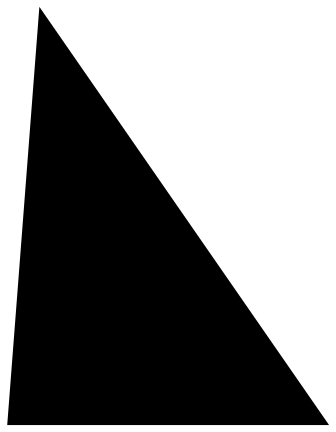
\includegraphics[scale=0.2]{tri}
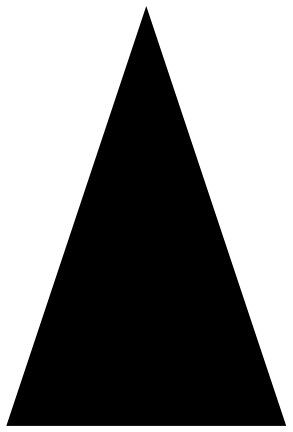
\includegraphics[scale=0.2]{etri}
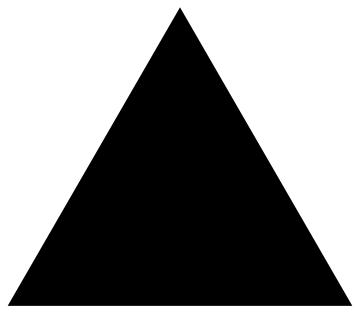
\includegraphics[scale=0.2]{rtri}
\end{center}

\ech
\end{frame}

\begin{frame}
\frametitle{\bch 对称性 \ech}
\bch

\begin{center}
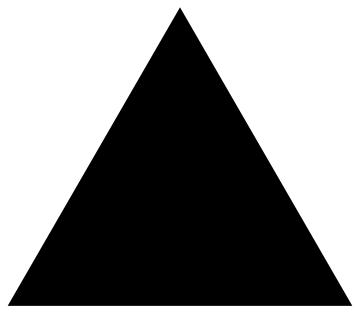
\includegraphics[scale=0.15]{rtri}
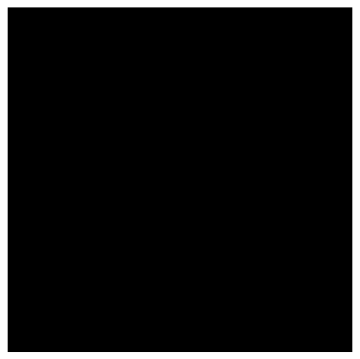
\includegraphics[scale=0.15]{pol4}
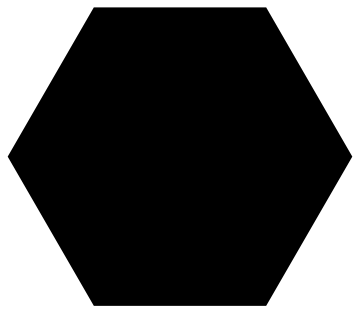
\includegraphics[scale=0.15]{pol6}
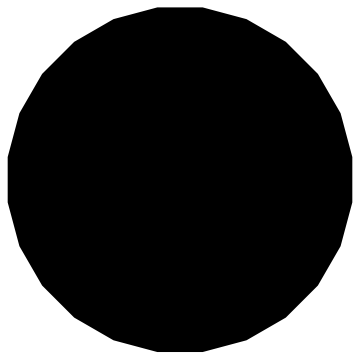
\includegraphics[scale=0.15]{pol24}

\includegraphics[scale=0.15]{cir}
\end{center}

\ech
\end{frame}

\begin{frame}
\frametitle{\bch 衡量对称性 \ech}
\bch
直观告诉我们可以分出图形对称性的大小,如何定量地去衡量?
\par
设$T$是对图形的一个操作,例如镜面反射和旋转。称$T$是一个对称操作,若操作前后图形完全相同。
\par
定义操作的乘法$T_2 T_1$为先进行操作1,再进行操作2。显然,若$T_1$和$T_2$都是对称操作,则它们的乘积也是对称操作(封闭性)。


\ech
\end{frame}

\begin{frame}
\frametitle{\bch 三角形的对称群 \ech}
\bch
记$I$为恒等操作(什么也不干),$R(\theta)$为逆时针旋转$\theta$角的操作,$r$为沿竖直的轴镜像反射的操作,则对三角形组,它们各自的所有对称操作组成的集合为
\begin{center}
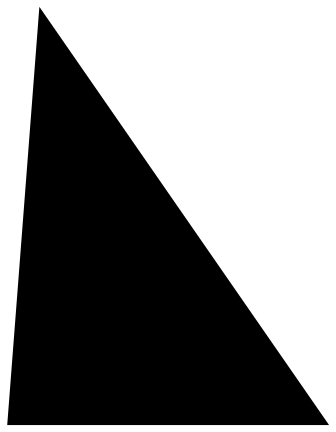
\includegraphics[scale=0.2]{tri}
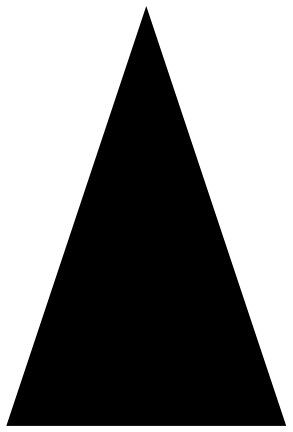
\includegraphics[scale=0.2]{etri}
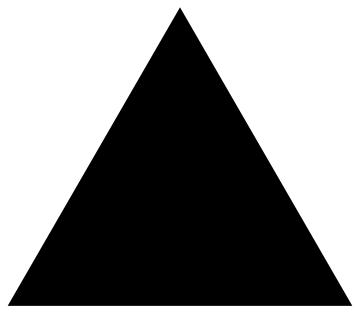
\includegraphics[scale=0.2]{rtri}
\end{center}
$$S_1 = \{I\},\ S_2 = \{I,r\},\ S_3 =\{I,r,R(120^\circ),R(240^\circ)\}$$

\ech
\end{frame}

\begin{frame}
\frametitle{\bch 正多边形的对称群 \ech}
\bch

\begin{center}
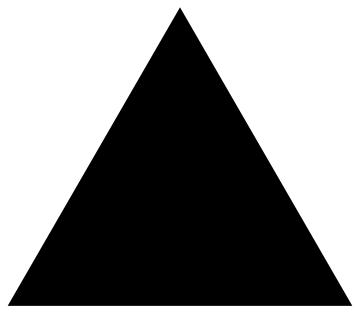
\includegraphics[scale=0.15]{rtri}
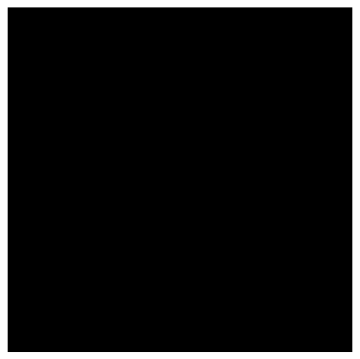
\includegraphics[scale=0.15]{pol4}
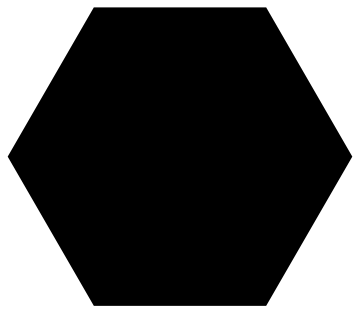
\includegraphics[scale=0.15]{pol6}
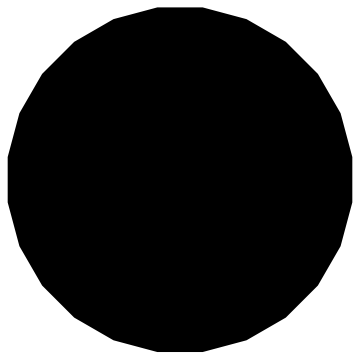
\includegraphics[scale=0.15]{pol24}

\includegraphics[scale=0.15]{cir}
\end{center}
正多边形各自的所有对称操作组成的集合为
$$D_3 = \{I,r,R(120^\circ),R(240^\circ)\},\ D_4 = \{I,r,R(90^\circ),R(180^\circ),R(270^\circ)\},$$
$$D_6 = \{I,r,R(60^\circ),R(120^\circ),R(180^\circ),R(240^\circ),R(300^\circ)\},$$
$$D_{24} = \{I,r,R(n\cdot 15^\circ)\},\ D_\infty = \{I,r,R(\theta) \ for \ \theta \in [0^\circ, 360^\circ)\}$$


\ech
\end{frame}

\begin{frame}
\frametitle{\bch 对称群 \ech}
\bch
群是一个对”乘法“封闭的集合$G$,并且
\begin{itemize}
\item 存在单位元$I \in G$,使得对任意其他元素$g \in G$都有$gI = Ig = g$。
\item 存在逆元,对任意元素$g \in G$,都存在一个元素$g^{-1}\in g$使得$g^{-1} g = gg^{-1} = I$。
\item 结合律成立,即$g_1 ( g_2 g_3) = (g_1 g_2) g_3$,乘法可以保持顺序任意加括号。
\end{itemize}
试验证刚才讨论的对称操作组成的集合满足上面三个要求,因此这些集合称为是图形对应的对称群。 
\par
经验总结:对称性越“大”,对称群的元素就越多。

\ech
\end{frame}

\section{Groups}
\begin{frame}
\frametitle{\bch 阿贝尔群 \ech}
\bch
群中的乘法一般是不可交换的,即$gh \not= hg$。若$gh = hg$对任意元素都成立,则称这个群是可交换群或阿贝尔群。

\ech
\end{frame}

\begin{frame}
\frametitle{\bch 群的其他实例 \ech}
\bch
三维空间旋转群$SO(3)$非阿贝尔,但$SO(2)$是阿贝尔群。
\par
方程$z^N = 1$在复数域的所有根构成阿贝尔群$Z_N$。
\par
$U(1) = \{ e^{i \theta},\ \theta \in \reals\}$是$Z_N$的连续极限。
\par
所有的$n$阶方阵构成非阿贝尔群。

\ech
\end{frame}

\begin{frame}
\frametitle{\bch 子群 \ech}
\bch
若(从集合角度)$H\subset G$,且$H$也构成群,则称$H$是$G$的子群。\par
例如$SO(2) \subset SO(3)$。


\ech
\end{frame}

\begin{frame}
\frametitle{\bch 直积 \ech}
\bch
两集合$F$和$G$的笛卡尔积定义为$F\otimes G = \{ (f,g) | f\in F, g \in G\}$。
若$F$和$G$构成群,则可以定义$F\otimes G$上的乘法
$$ (f_1,g_1) (f_2,g_2) = (f_1 f_2,g_1g_2)$$
这显然使得$F\otimes G$构成群,称为$F$和$G$的直积。
\par
显然有$F,G \subset F \otimes G$。


\ech
\end{frame}



\section{Discrete Groups}
\begin{frame}
\frametitle{\bch 离散群 \ech}
\bch
元素有限的群称为有限群,元素可数的群称为离散群。\par
循环群,拉格朗日定理,乘法表,表示论,同态和同构,不变子群和派生子群,商群......看黑板,懒得打字了。


\ech
\end{frame}



























\end{document}
